\documentclass[conference,onecolumn]{IEEEtran}
\IEEEoverridecommandlockouts
\usepackage{cite}
\usepackage{amsmath,amssymb,amsfonts}
\usepackage{algorithmic}
\usepackage{graphicx}
\usepackage{listings}
\usepackage{float}
\usepackage{textcomp}
\usepackage{gensymb}
\usepackage{xcolor}
\usepackage[spanish]{babel}
\def\BibTeX{{\rm B\kern-.05em{\sc i\kern-.025em b}\kern-.08em
    T\kern-.1667em\lower.7ex\hbox{E}\kern-.125emX}}

% --- Estilo de listados de codigo (borde verde, fondo blanco) ---
\definecolor{listinggreen}{RGB}{0,130,0}
\lstdefinestyle{tallerstyle}{backgroundcolor=\color{white},basicstyle=\ttfamily\footnotesize,breaklines=true,frame=single,rulecolor=\color{listinggreen},frameround=ffff,framesep=4pt,xleftmargin=6pt,xrightmargin=6pt,commentstyle=\color{gray},keywordstyle=\color{blue!70!black},stringstyle=\color{red!60!black},showstringspaces=false,columns=flexible,keepspaces=true,numbers=left,numberstyle=\tiny\color{gray}}
\lstset{style=tallerstyle}

\begin{document}

\title{Pr\'actica 3: Diversidad en recepci\'on mediante combinaci\'on por relaci\'on m\'axima (MRC) sobre un sistema OFDM conforme a LTE}

\author{\IEEEauthorblockN{Tyrone Miguel Novillo Bravo}
\IEEEauthorblockA{Facultad de Ingenier\'ia\\
Departamento de Telecomunicaciones\\
Universidad de Cuenca\\
tyrone.novillo@ucuenca.edu.ec}
\and
\IEEEauthorblockN{Freddy Eduardo L\'opez Padilla}
\IEEEauthorblockA{Facultad de Ingenier\'ia\\
Departamento de Telecomunicaciones\\
Universidad de Cuenca\\
freddy.lopez@ucuenca.edu.ec}}

\maketitle

\begin{abstract}
Este trabajo implementa y eval\'ua la diversidad en recepci\'on con combinaci\'on por relaci\'on m\'axima (\textit{Maximum-Ratio Combining}, MRC) sobre el simulador OFDM de las pr\'acticas anteriores. El transmisor no cambia: env\'ia una sola se\~nal OFDM. El receptor, en cambio, dispone de $N_R$ antenas; la misma se\~nal llega por $N_R$ canales Pedestrian A independientes ---cada uno con su propio desvanecimiento de Rayleigh y su propio ruido AWGN--- y se combina por subportadora con MRC, ponderando cada rama por el conjugado de su respuesta de canal $H_m[k]$. Al disponer del canal generado por el propio simulador (CSI perfecta), no se requiere estimaci\'on de canal. La evaluaci\'on se centra en el an\'alisis de resultados: se transmite la imagen de Lena con $2$, $4$ y $8$ antenas, se compara la constelaci\'on recibida antes y despu\'es de la combinaci\'on, y se obtienen las curvas BER frente a SNR para las modulaciones QPSK, 16-QAM y 64-QAM mediante un an\'alisis de Monte Carlo con intervalos de confianza al $95\%$ ($t$ de Student). Los resultados confirman la ganancia de diversidad de orden $N_R$: cada antena a\~nadida desplaza la curva BER hacia abajo y a la izquierda, mejorando la SNR efectiva en proporci\'on al n\'umero de antenas.
\end{abstract}

\begin{IEEEkeywords}
Diversidad en recepci\'on, MRC, MIMO, OFDM, LTE, BER, ganancia de diversidad, desvanecimiento de Rayleigh, Monte Carlo.
\end{IEEEkeywords}

\section*{Objetivos}

\textbf{Objetivo general:} Implementar y evaluar la diversidad en recepci\'on con MRC sobre la cadena OFDM de las pr\'acticas anteriores, verificando que el aumento del n\'umero de antenas receptoras reduce la tasa de error de bit (BER) gracias a la ganancia de diversidad.

\textbf{Objetivos espec\'ificos:}
\begin{itemize}
    \item Modelar un receptor de $N_R$ antenas en el que la misma se\~nal transmitida atraviesa $N_R$ canales Pedestrian A independientes con ruido independiente.
    \item Implementar la combinaci\'on MRC por subportadora reutilizando la respuesta de canal conocida $H_m[k]$, sin estimaci\'on de canal.
    \item Comparar visualmente, mediante la transmisi\'on de la imagen de Lena y la constelaci\'on recibida, el efecto de combinar $2$, $4$ y $8$ antenas.
    \item Caracterizar la ganancia de diversidad mediante curvas BER frente a SNR (Monte Carlo, IC al $95\%$) para QPSK, 16-QAM y 64-QAM.
\end{itemize}

\section{Introducci\'on}

En un canal m\'ovil con desvanecimiento, la calidad del enlace var\'ia de forma aleatoria: en los instantes (o subportadoras) en los que el canal sufre un desvanecimiento profundo, la SNR cae y aparecen errores. Una de las t\'ecnicas m\'as eficaces y simples para combatir este efecto es la \emph{diversidad en recepci\'on}, que consiste en dotar al receptor de varias antenas suficientemente separadas para que sus canales sean estad\'isticamente independientes \cite{vazquezrodas_lte,dahlman2014lte}. La probabilidad de que todas las ramas sufran un desvanecimiento profundo \emph{a la vez} disminuye r\'apidamente con el n\'umero de antenas, de modo que combinando adecuadamente las se\~nales recibidas se obtiene un enlace mucho m\'as robusto.

La estrategia \'optima de combinaci\'on cuando el deterioro dominante es el ruido es la combinaci\'on por relaci\'on m\'axima (MRC), que maximiza la SNR tras la combinaci\'on \cite{brennan2003linear,goldsmith2005wireless}. En este trabajo se a\~nade al simulador una tercera pesta\~na que reutiliza \'integramente el transmisor OFDM y modifica \'unicamente el receptor para incorporar MRC con $N_R\in\{2,4,8\}$ antenas. Como el modelo de canal se genera dentro del propio c\'odigo, su respuesta en frecuencia est\'a disponible en el receptor y se emplea directamente como informaci\'on de estado de canal (CSI) perfecta, evitando la etapa de estimaci\'on. El an\'alisis se enfoca en los resultados: la recuperaci\'on de una imagen, la constelaci\'on antes y despu\'es de combinar, y las curvas BER frente a SNR.

\section{Marco te\'orico}

\subsection{Diversidad en recepci\'on y combinaci\'on lineal}

Con $N_R$ antenas, y asumiendo que en cada subportadora el canal es de banda angosta (desvanecimiento plano, propiedad que OFDM garantiza al dividir la banda en subportadoras estrechas), la se\~nal recibida en la antena $m$ puede escribirse como
\begin{equation}
r_m = h_m\, s + n_m, \qquad m = 1,\dots,N_R, \label{eq:rx}
\end{equation}
donde $s$ es el s\'imbolo transmitido, $h_m$ la ganancia compleja del canal de la rama $m$ y $n_m$ su ruido AWGN. El receptor combina linealmente las ramas mediante pesos complejos $w_m^{*}$: $\;y=\sum_{m=1}^{N_R} w_m^{*}\, r_m$ \cite{vazquezrodas_lte}.

\subsection{Combinaci\'on por relaci\'on m\'axima (MRC)}

Para maximizar la SNR tras la combinaci\'on, los pesos deben elegirse iguales a las ganancias de canal, $\mathbf{w}_{\mathrm{MRC}}=\mathbf{h}$ \cite{brennan2003linear,tse2005fundamentals}. Con esta elecci\'on, la estimaci\'on del s\'imbolo por subportadora en el sistema OFDM es
\begin{equation}
\hat{X}[k]=\frac{\sum_{m=1}^{N_R} H_m^{*}[k]\,Y_m[k]}{\sum_{m=1}^{N_R} |H_m[k]|^{2}}, \label{eq:mrc}
\end{equation}
donde $Y_m[k]$ es la se\~nal recibida en la subportadora $k$ de la antena $m$ y $H_m[k]$ su respuesta de canal. Los pesos $H_m^{*}[k]$ cumplen dos funciones \cite{vazquezrodas_lte}: \emph{(i)} rotan en fase cada rama para compensar la fase del canal, de modo que las se\~nales se suman de forma \emph{coherente}; y \emph{(ii)} ponderan cada rama en proporci\'on a su ganancia, dando m\'as peso a las antenas con mejor canal. Si las antenas no est\'an correladas, la combinaci\'on aporta una diversidad de orden $N_R$ y la SNR efectiva crece aproximadamente en proporci\'on al n\'umero de antenas (ganancia de array $\sim 10\log_{10} N_R$ dB) \cite{vazquezrodas_lte,goldsmith2005wireless}.

\subsection{Cadena reutilizada y modelo de canal}

El transmisor (mapeo QAM con codificaci\'on Gray, inserci\'on de pilotos, IFFT con prefijo c\'iclico) y el modelo de canal son los de las pr\'acticas anteriores. Cada rama emplea una realizaci\'on \emph{independiente} del canal Pedestrian A (ITU-R M.1225), de cuatro taps con desvanecimiento de Rayleigh (Tabla~\ref{tab:pedA}) \cite{ituR1225,rappaport2002}, y un ruido AWGN independiente calibrado al mismo valor de SNR por antena. Esta independencia entre ramas es la condici\'on que habilita la ganancia de diversidad. La validaci\'on estad\'istica de las curvas BER se realiza mediante Monte Carlo con intervalos de confianza basados en la distribuci\'on $t$ de Student \cite{montgomery2011}.

\begin{table}[H]
    \renewcommand{\arraystretch}{1.2}
    \caption{Perfil potencia-retardo del modelo Pedestrian A \cite{ituR1225}.}
    \label{tab:pedA}
    \centering
    \begin{tabular}{ccc}
        \hline
        \textbf{Tap} & \textbf{Retardo (ns)} & \textbf{Potencia (dB)} \\
        \hline
        1 & 0   & 0       \\
        2 & 110 & -9{,}7  \\
        3 & 190 & -19{,}2 \\
        4 & 410 & -22{,}8 \\
        \hline
    \end{tabular}
\end{table}

\section{Implementaci\'on del receptor MRC}

La \'unica modificaci\'on respecto a la cadena anterior est\'a en el receptor: se a\~nadi\'o el par\'ametro \texttt{n\_rx} a la funci\'on \texttt{cadena\_tx\_rx}. Con \texttt{n\_rx}${=}1$ el comportamiento es el de un receptor cl\'asico de una antena con ecualizaci\'on Zero-Forcing; con \texttt{n\_rx}${>}1$, el mismo s\'imbolo OFDM se hace pasar por \texttt{n\_rx} canales y ruidos independientes y se combinan seg\'un \eqref{eq:mrc}, reutilizando las funciones ya existentes \texttt{generar\_canal\_pedestrian\_a}, \texttt{modulacion\_ofdm}, \texttt{agregar\_ruido\_awgn} y \texttt{demodulacion\_ofdm}.

\begin{lstlisting}[language=Python]
num = np.zeros(n_sc, dtype=complex)   # numerador MRC:  sum conj(H_m) * Y_m
den = np.zeros(n_sc, dtype=float)     # denominador:    sum |H_m|^2
for m in range(n_rx):
    H_m = generar_canal_pedestrian_a(n_fft, fs, indices_fft, rng)  # canal independiente
    senal_canal, _ = modulacion_ofdm(rejilla * H_m, n_fft, n_cp)
    senal_rx = agregar_ruido_awgn(senal_canal, snr_db, rng)        # ruido independiente
    rejilla_rx_m = demodulacion_ofdm(senal_rx, indices_fft, n_fft, n_cp, n_sc)
    num += np.conj(H_m) * rejilla_rx_m    # combinacion coherente (rota fase y pondera)
    den += np.abs(H_m) ** 2
rejilla_eq = num / (den + 1e-12)          # estimacion MRC de X[k]
\end{lstlisting}

N\'otese que la divisi\'on por $\sum_m |H_m|^2$ deja la estimaci\'on en la escala del s\'imbolo transmitido, por lo que la combinaci\'on MRC sustituye e incorpora a la ecualizaci\'on: no se requiere un paso adicional de Zero-Forcing.

\section{Evaluaci\'on -- An\'alisis de resultados}

\subsection{Configuraci\'on y metodolog\'ia}

Las pruebas usan la configuraci\'on $BW{=}5$~MHz, $\Delta f{=}15$~kHz y CP normal ($N_{SC}{=}300$, $N_{FFT}{=}512$, $f_s{=}7{,}680$~MHz). La SNR indicada es \emph{por antena}: cada rama recibe la se\~nal a la misma SNR objetivo, de modo que la mejora observada proviene exclusivamente de la combinaci\'on y no de un aumento de potencia. Las curvas BER se obtienen por Monte Carlo con $10$ corridas independientes por punto e intervalos de confianza al $95\%$. La transmisi\'on de imagen emplea la fotograf\'ia est\'andar de Lena reescalada a $96\times96$ p\'ixeles.

\subsection{Recuperaci\'on de imagen con $2$, $4$ y $8$ antenas}

La Fig.~\ref{fig:lena} muestra la imagen de Lena recuperada con 16-QAM a una SNR baja de $6$~dB por antena, para $2$, $4$ y $8$ antenas. El efecto de la diversidad es evidente a simple vista: con $2$ antenas la imagen presenta un moteado intenso (BER ${=}5{,}4\times10^{-2}$); con $4$ antenas el ruido se reduce de forma notable (BER ${=}2{,}2\times10^{-2}$); y con $8$ antenas la imagen es pr\'acticamente limpia (BER ${=}4{,}2\times10^{-3}$). Cada duplicaci\'on del n\'umero de antenas reduce la BER en m\'as de la mitad, ilustrando directamente la ganancia de diversidad que se obtiene combinando las se\~nales de las distintas ramas.

\begin{figure}[H]
\centering
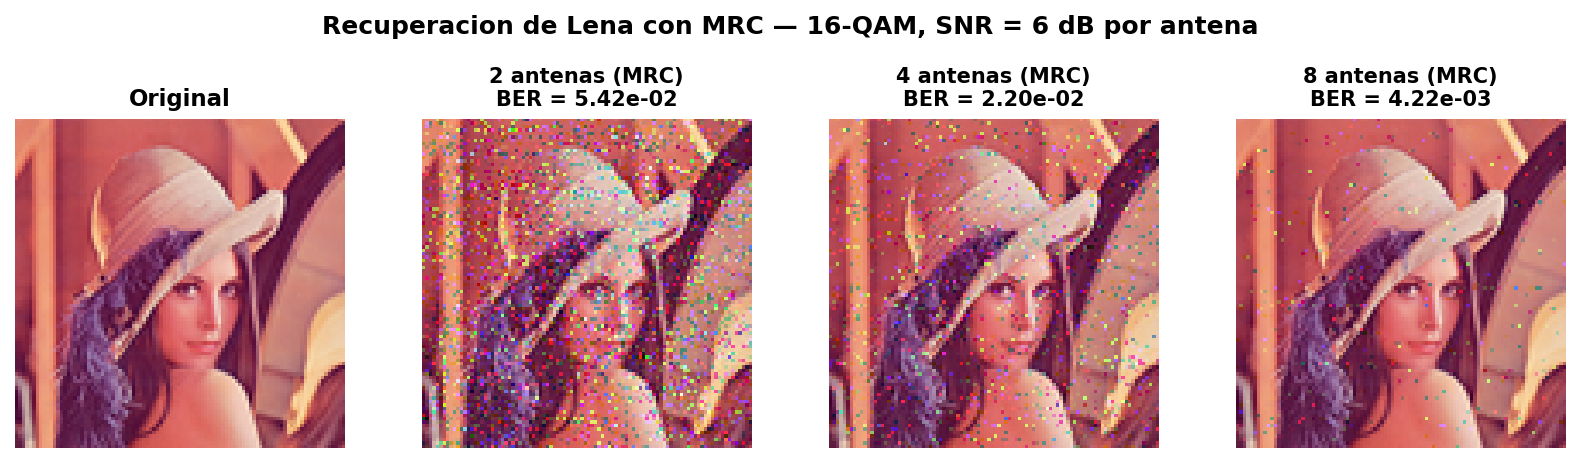
\includegraphics[width=0.98\textwidth]{img/lena_mrc.png}
\caption{Imagen de Lena recuperada con MRC (16-QAM, SNR${=}6$~dB por antena) para $2$, $4$ y $8$ antenas. A mayor n\'umero de antenas, menor BER y mejor calidad de imagen.}
\label{fig:lena}
\end{figure}

\subsection{Constelaci\'on antes y despu\'es de la combinaci\'on MRC}

La Fig.~\ref{fig:const} compara la constelaci\'on de 16-QAM recibida a $8$~dB por antena antes y despu\'es de MRC. A la izquierda se muestra la se\~nal de una sola antena tras la ecualizaci\'on Zero-Forcing: el ruido ---amplificado en las subportadoras con desvanecimiento profundo--- dispersa tanto los s\'imbolos que los $16$ puntos de la ret\'icula apenas se distinguen. A la derecha, la combinaci\'on de las $8$ antenas concentra los s\'imbolos en torno a las posiciones ideales (cruces negras), formando $16$ n\'ucleos bien definidos. La figura visualiza las dos acciones de MRC: la alineaci\'on de fase (suma coherente) y la ponderaci\'on por la ganancia de canal, que en conjunto reducen dr\'asticamente la varianza del ruido en el s\'imbolo combinado.

\begin{figure}[H]
\centering
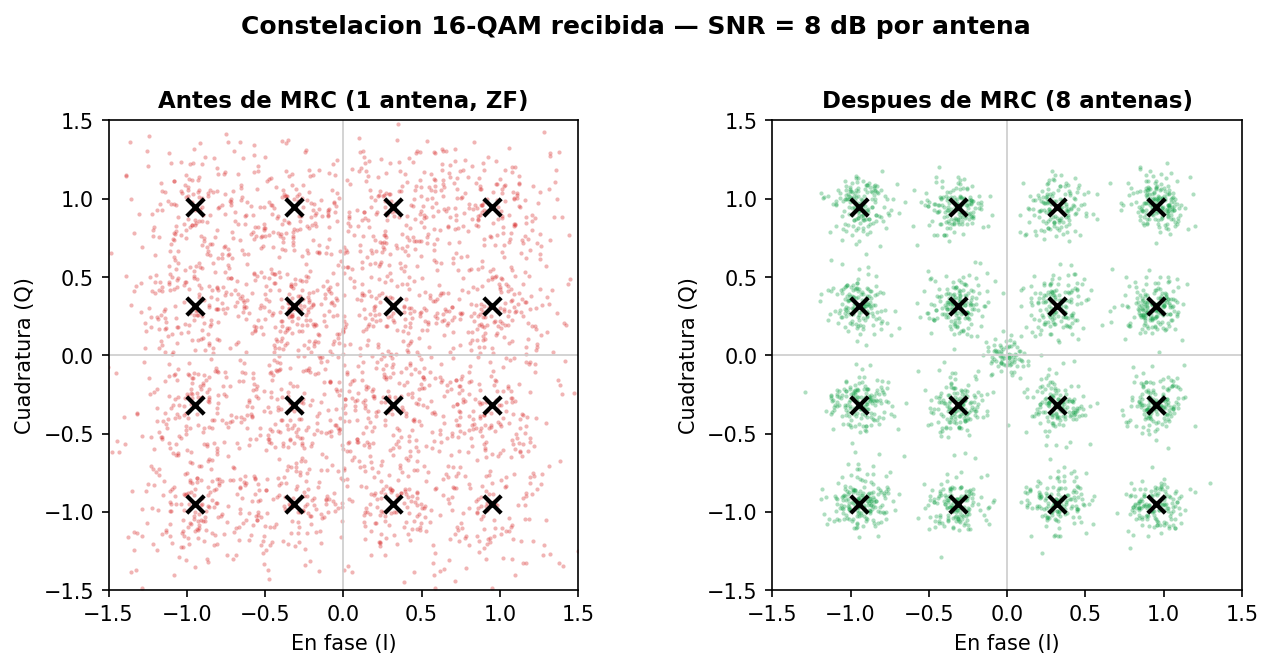
\includegraphics[width=0.92\textwidth]{img/constelacion_mrc.png}
\caption{Constelaci\'on de 16-QAM recibida (SNR${=}8$~dB por antena). Izquierda: una sola antena (Zero-Forcing), nube muy dispersa. Derecha: $8$ antenas combinadas con MRC, s\'imbolos agrupados en torno a los puntos ideales.}
\label{fig:const}
\end{figure}

\subsection{Curvas BER frente a SNR: ganancia de diversidad}

La Fig.~\ref{fig:montecarlo} presenta el resultado central de la pr\'actica: las curvas BER frente a SNR para $2$, $4$ y $8$ antenas, en las tres modulaciones. En los tres casos las curvas mantienen el mismo orden ---a igualdad de SNR, m\'as antenas implican menor BER--- y, adem\'as, su pendiente se hace m\'as pronunciada al aumentar $N_R$, lo que es la firma caracter\'istica del aumento del orden de diversidad. Para 16-QAM a $8$~dB, la BER pasa de $3{,}1\times10^{-2}$ con $2$ antenas a $7{,}4\times10^{-3}$ con $4$ y a $7{,}9\times10^{-4}$ con $8$, es decir, aproximadamente un orden de magnitud de mejora al pasar de $2$ a $8$ antenas. La modulaci\'on robusta QPSK alcanza el piso de error ya a SNR bajas incluso con pocas antenas, mientras que 64-QAM, mucho m\'as exigente, parte de una BER alta pero se beneficia igualmente de la diversidad: a $12$~dB su BER cae de $4{,}8\times10^{-2}$ ($2$ antenas) a $3{,}8\times10^{-3}$ ($8$ antenas). El desplazamiento de las curvas hacia la izquierda al a\~nadir antenas es coherente con la ganancia de array de $\sim 10\log_{10} N_R$ dB prevista por la teor\'ia \cite{vazquezrodas_lte}.

\begin{figure}[H]
\centering
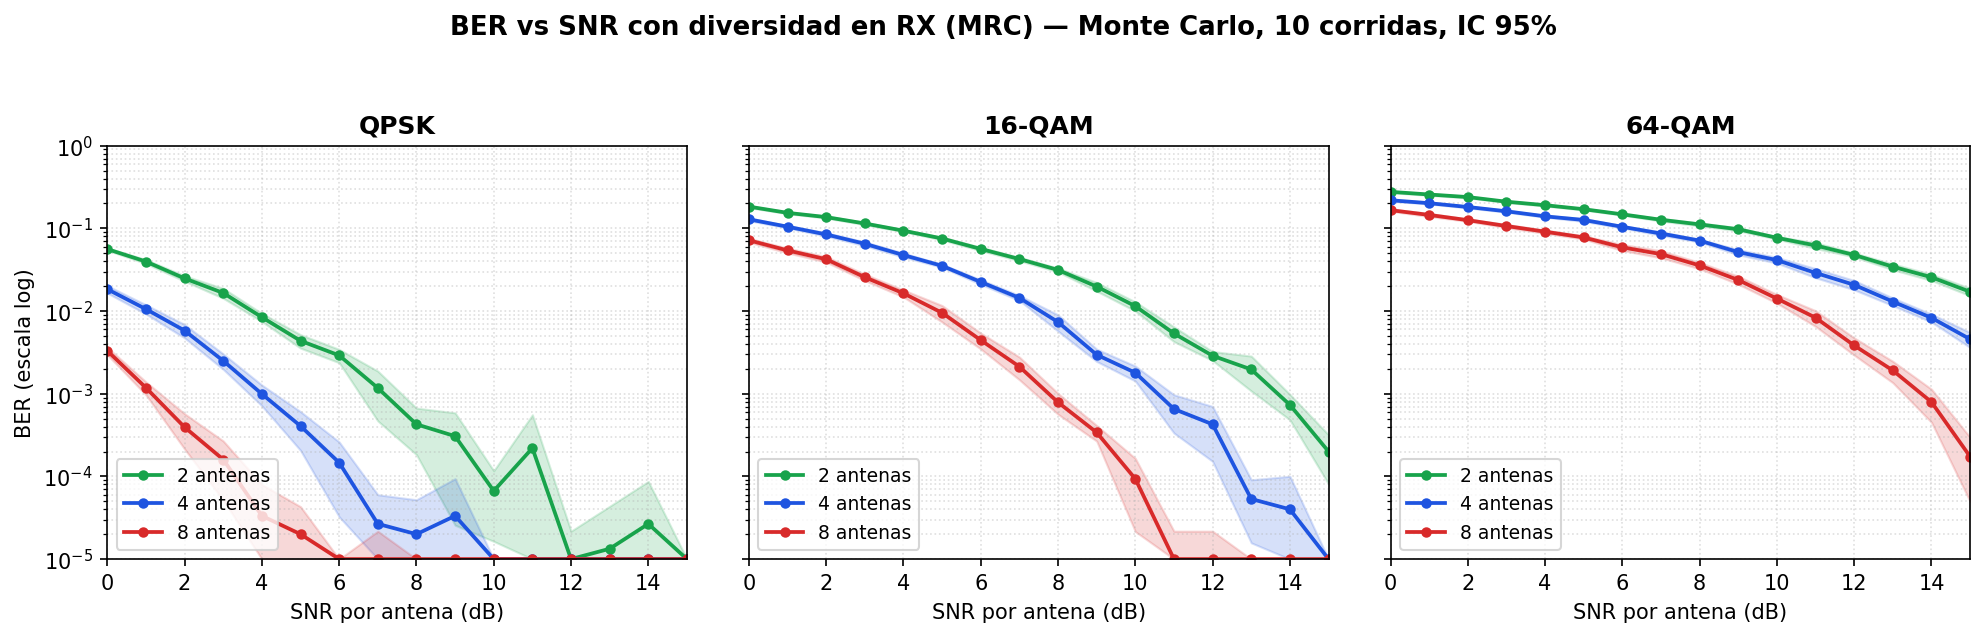
\includegraphics[width=0.98\textwidth]{img/montecarlo_mrc.png}
\caption{BER frente a SNR por antena con diversidad en RX (MRC), para QPSK, 16-QAM y 64-QAM. Cada panel muestra las curvas de $2$, $4$ y $8$ antenas con su banda de confianza al $95\%$ (Monte Carlo, $10$ corridas por punto). M\'as antenas $\Rightarrow$ curva m\'as baja y de mayor pendiente (mayor orden de diversidad).}
\label{fig:montecarlo}
\end{figure}

\section{Conclusiones}

Se implement\'o la diversidad en recepci\'on con MRC reutilizando \'integramente el transmisor OFDM de las pr\'acticas anteriores y modificando \'unicamente el receptor. La incorporaci\'on requiri\'o un solo cambio funcional ---combinar por subportadora las $N_R$ ramas mediante $\hat{X}[k]=\sum_m H_m^{*}[k]Y_m[k]/\sum_m |H_m[k]|^2$---, aprovechando que el canal generado por el simulador est\'a disponible como CSI perfecta, lo que hace innecesaria la estimaci\'on de canal.

Los resultados verifican el objetivo de la pr\'actica. La transmisi\'on de la imagen de Lena mostr\'o de forma directa c\'omo la calidad mejora al pasar de $2$ a $8$ antenas (BER de $5{,}4\times10^{-2}$ a $4{,}2\times10^{-3}$ a $6$~dB), y la constelaci\'on evidenci\'o c\'omo MRC concentra los s\'imbolos dispersos de una sola antena en n\'ucleos compactos. El an\'alisis de Monte Carlo confirm\'o cuantitativamente la ganancia de diversidad: para las tres modulaciones, cada antena a\~nadida desplaza la curva BER hacia abajo y a la izquierda, con una mejora de aproximadamente un orden de magnitud al pasar de $2$ a $8$ antenas y una pendiente creciente que refleja el aumento del orden de diversidad. Se confirma as\'i el principio te\'orico: combinando coherentemente se\~nales de canales independientes, MRC incrementa la SNR efectiva en proporci\'on al n\'umero de antenas receptoras, mejorando la robustez del enlace sin modificar el transmisor.

\bibliographystyle{IEEEtran}
\bibliography{referencias}

\clearpage
\onecolumn
\newpage
\section*{Anexos}

\begin{figure}[H]
    \centering
    
\includegraphics[width=0.22\textwidth]{img/qr_sitio.png}
    \caption{C\'odigo QR del simulador desplegado: \texttt{https://ofdm.tesisucuenca.com}}
    \label{fig:qrsitio}
\end{figure}

\begin{figure}[H]
    \centering
    
\includegraphics[width=0.22\textwidth]{img/qr_repo.png}
    \caption{C\'odigo QR del repositorio del proyecto: \texttt{https://github.com/thyron001/ofdm}}
    \label{fig:qrrepo}
\end{figure}

\end{document}
